\documentclass{book}

% References
\usepackage[colorlinks=true]{hyperref}
\usepackage{url}

% For trees
% http://ftp.math.purdue.edu/mirrors/ctan.org/macros/latex/contrib/genealogytree/genealogytree.pdf
\usepackage[all]{genealogytree}

% Remove chapter N text
\usepackage[pagestyles]{titlesec}
\titleformat{\chapter}[display]{\normalfont\bfseries}{}{0pt}{\Huge}
\newpagestyle{mystyle}
{\sethead[\thepage][][\chaptertitle]{}{}{\thepage}}
\pagestyle{mystyle}
\titlespacing*{\chapter}{0pt}{0pt}{20pt}


% Timeline
\usepackage{array, booktabs}
\usepackage{graphicx}
\newcommand{\foo}{\makebox[0pt]{\textbullet}\hskip-0.5pt\vrule width 1pt\hspace{\labelsep}}


\begin{document}

\title{Family Tree}
\author{Steven Elsworth}
\maketitle

\chapter{How does it work?}
This interactive pdf contains a sample family tree. Each member of the family has their own chapter of the book containing:
\begin{itemize}
\item Immediate family tree: The small tree contains their siblings, parents, spouse and children. Each member of the tree with their own chapter can be accessed via the hyperlink.
\item Timeline: A timeline breakdown of key events in their life. 
\item Data: A list of links which opens external files showing evidence. This can include pdfs/jpeg/png of birth certificates, census records, images or even web links.
\end{itemize} 

This document works best when opened with Adobe Acrobat Reader.

\vspace{1in}
Note: if text appears \color{red} red \color{black} then it is a hyperlink.

\chapter{Child1}
\label{Child1}
\begin{center}
\huge{2000 --}
\end{center}

\vspace{1in}

\begin{center}
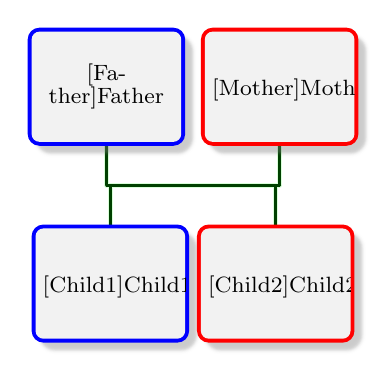
\begin{tikzpicture}
\genealogytree[template=signpost]{ parent{
        g[male]{\hyperref[Child1]{Child1}}
        c[female]{\hyperref[Child2]{Child2}}
        p[male]{\hyperref[Father]{Father}}
        p[female]{\hyperref[Mother]{Mother}}
} }
\end{tikzpicture}
\end{center}

\newpage
\section{Timeline}
\begin{table}[h]
\renewcommand\arraystretch{1.4}
\begin{tabular}{@{\,}r <{\hskip 2pt} !{\foo} >{\raggedright\arraybackslash}p{20cm}}
\addlinespace[1.5ex]
1st January 2000 & BORN in ...\\
1st January 2001 & Baptised in ... \\
\end{tabular}
\end{table}

\section{Data}
\begin{itemize}
\item \href{run:people/Child1/sample.pdf}{Sample pdf}
\item \href{run:people/Child1/sample.png}{Sample png}
\item \href{https://github.com/StevenElsworth?tab=repositories}{Sample link} 
\end{itemize}

\chapter{Child2}
\label{Child2}
\begin{center}
\huge{2000 --}
\end{center}

\vspace{1in}

\begin{center}
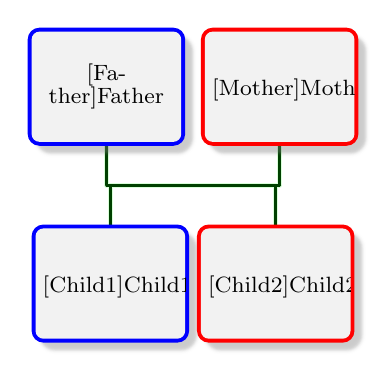
\begin{tikzpicture}
\genealogytree[template=signpost]{ parent{
        c[male]{\hyperref[Child1]{Child1}}
        g[female]{\hyperref[Child2]{Child2}}
        p[male]{\hyperref[Father]{Father}}
        p[female]{\hyperref[Mother]{Mother}}
} }
\end{tikzpicture}
\end{center}

\newpage
\section{Timeline}
\begin{table}[h]
\renewcommand\arraystretch{1.4}
\begin{tabular}{@{\,}r <{\hskip 2pt} !{\foo} >{\raggedright\arraybackslash}p{20cm}}
\addlinespace[1.5ex]
1st January 2000 & BORN in ...\\
1st January 2001 & Baptised in ... \\
\end{tabular}
\end{table}

\section{Data}
\begin{itemize}
\item \href{run:people/Child2/sample.pdf}{Sample pdf}
\item \href{run:people/Child2/sample.png}{Sample png}
\item \href{https://github.com/StevenElsworth?tab=repositories}{Sample link} 
\end{itemize}

\chapter{Father} 
\label{Father}
\begin{center}
\huge{1980 --}
\end{center}

\vspace{1in}

\begin{center}
 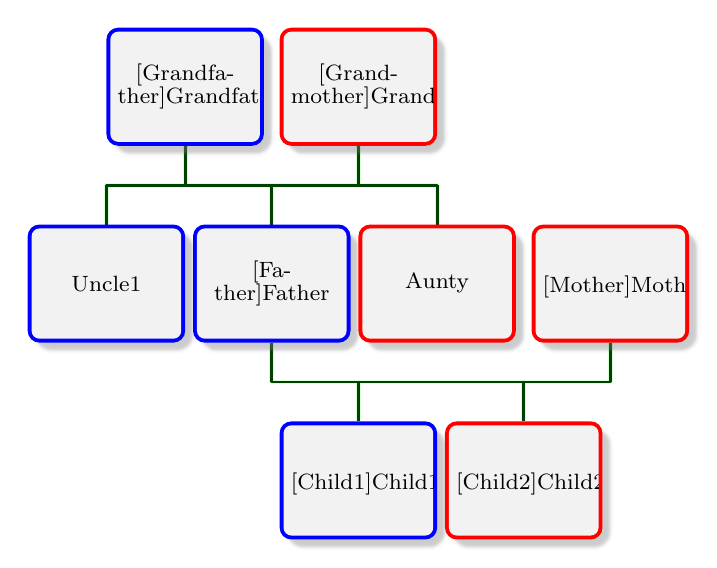
\begin{tikzpicture} \genealogytree[template=signpost]{
    parent{
      g[male]{\hyperref[Child1]{Child1}}
      c[female]{\hyperref[Child2]{Child2}}
      parent{
        c[male]{Uncle1}
        g[male]{\hyperref[Father]{Father}}
        c[female]{Aunty}
        p[male]{\hyperref[Grandfather]{Grandfather}}
        p[female]{\hyperref[Grandmother]{Grandmother}}
}
      p[female]{\hyperref[Mother]{Mother}}
    }
  }
\end{tikzpicture}
\end{center}

\newpage
\section{Timeline}
\begin{table}[h]
\renewcommand\arraystretch{1.4}
\begin{tabular}{@{\,}r <{\hskip 2pt} !{\foo} >{\raggedright\arraybackslash}p{20cm}}
\addlinespace[1.5ex]
1st January 1980 & BORN in ...\\
1st January 1981 & Baptised in ... \\
\end{tabular}
\end{table}

\section{Data}
\begin{itemize}
\item \href{run:people/Child1/sample.pdf}{Sample pdf}
\item \href{run:people/Child1/sample.png}{Sample png}
\item \href{https://github.com/StevenElsworth?tab=repositories}{Sample link} 
\end{itemize}

\chapter{Mother} 
\label{Mother}
\begin{center}
\huge{1982 --}
\end{center}

\vspace{1in}

\begin{center}
 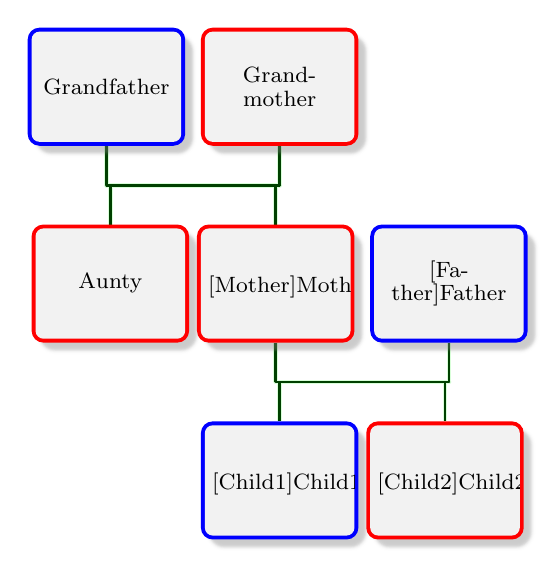
\begin{tikzpicture} \genealogytree[template=signpost]{
    parent{
      g[male]{\hyperref[Child1]{Child1}}
      c[female]{\hyperref[Child2]{Child2}}
      parent{
        c[female]{Aunty}
        g[female]{\hyperref[Mother]{Mother}}
        p[male]{Grandfather}
        p[female]{Grandmother}
}
      p[male]{\hyperref[Father]{Father}}
    }
  }
\end{tikzpicture}
\end{center}

\newpage
\section{Timeline}
\begin{table}[h]
\renewcommand\arraystretch{1.4}
\begin{tabular}{@{\,}r <{\hskip 2pt} !{\foo} >{\raggedright\arraybackslash}p{20cm}}
\addlinespace[1.5ex]
1st January 1982 & BORN in ...\\
1st January 1983 & Baptised in ... \\
\end{tabular}
\end{table}

\section{Data}
\begin{itemize}
\item \href{run:people/Child1/sample.pdf}{Sample pdf}
\item \href{run:people/Child1/sample.png}{Sample png}
\item \href{https://github.com/StevenElsworth?tab=repositories}{Sample link} 
\end{itemize}

\chapter{Grandfather} 
\label{Grandfather}
\begin{center}
\huge{1960 --}
\end{center}

\vspace{1in}

\begin{center}
 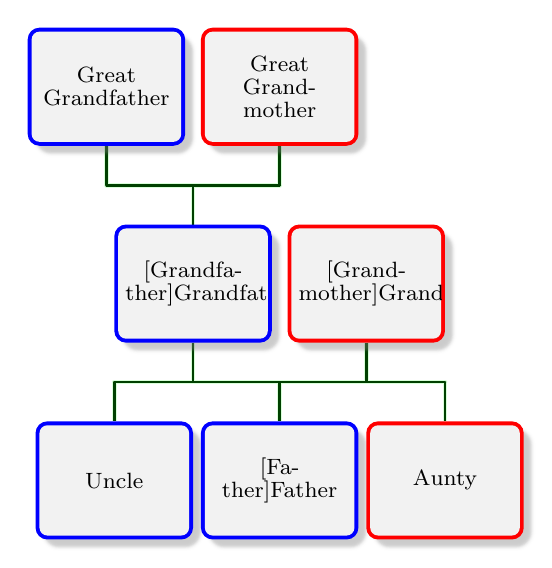
\begin{tikzpicture} \genealogytree[template=signpost]{
    parent{
	  c[male]{Uncle}
      g[male]{\hyperref[Father]{Father}}
      c[female]{Aunty}
      parent{
        g[male]{\hyperref[Grandfather]{Grandfather}}
        p[male]{Great Grandfather}
        p[female]{Great Grandmother}
}
      p[female]{\hyperref[Grandmother]{Grandmother}}
    }
  }
\end{tikzpicture}
\end{center}

\newpage
\section{Timeline}
\begin{table}[h]
\renewcommand\arraystretch{1.4}
\begin{tabular}{@{\,}r <{\hskip 2pt} !{\foo} >{\raggedright\arraybackslash}p{20cm}}
\addlinespace[1.5ex]
1st January 1960 & BORN in ...\\
1st January 1961 & Baptised in ... \\
\end{tabular}
\end{table}

\section{Data}
\begin{itemize}
\item \href{run:people/Child1/sample.pdf}{Sample pdf}
\item \href{run:people/Child1/sample.png}{Sample png}
\item \href{https://github.com/StevenElsworth?tab=repositories}{Sample link} 
\end{itemize}

\chapter{Grandmother} 
\label{Grandmother}
\begin{center}
\huge{1962 - 2010}
\end{center}

\vspace{1in}

\begin{center}
 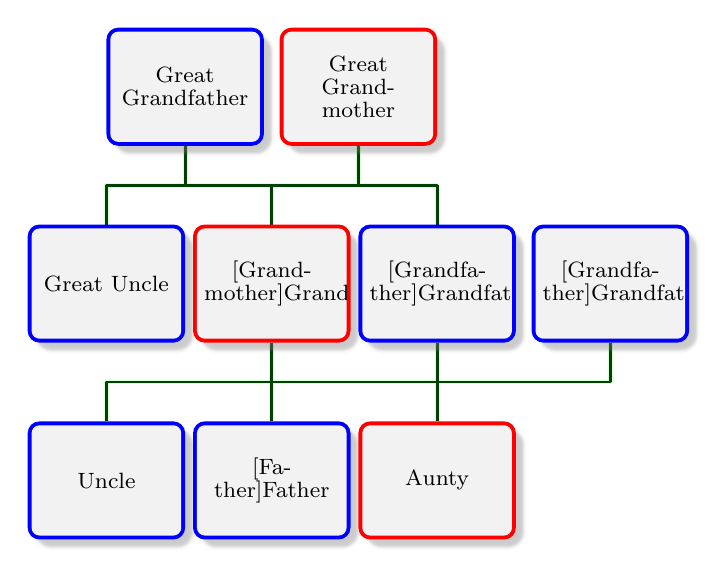
\begin{tikzpicture} \genealogytree[template=signpost]{
    parent{
	  c[male]{Uncle}
      g[male]{\hyperref[Father]{Father}}
      c[female]{Aunty}
      parent{
        c[male]{Great Uncle}
        g[female]{\hyperref[Grandmother]{Grandmother}}
        g[male]{\hyperref[Grandfather]{Grandfather}}
        p[male]{Great Grandfather}
        p[female]{Great Grandmother}
}
      p[male]{\hyperref[Grandfather]{Grandfather}}
    }
  }
\end{tikzpicture}
\end{center}

\newpage
\section{Timeline}
\begin{table}[h]
\renewcommand\arraystretch{1.4}
\begin{tabular}{@{\,}r <{\hskip 2pt} !{\foo} >{\raggedright\arraybackslash}p{20cm}}
\addlinespace[1.5ex]
1st January 1962 & BORN in ...\\
1st January 1963 & Baptised in ... \\
\end{tabular}
\end{table}

\section{Data}
\begin{itemize}
\item \href{run:people/Child1/sample.pdf}{Sample pdf}
\item \href{run:people/Child1/sample.png}{Sample png}
\item \href{https://github.com/StevenElsworth?tab=repositories}{Sample link} 
\end{itemize}

\end{document}
